\documentclass[fleqn,12pt]{olplainarticle}
\usepackage{graphicx}
\graphicspath{ {./} }
% Use option lineno for line numbers 
\renewcommand{\baselinestretch}{1.3}

\title{Docker in Software Architecture – Technology brief (c)}

\author[1]{Daniel Koch}
\author[2]{Sebastian Sergelius}
\affil[1]{daniel.koch@helsinki.fi}
\affil[2]{sebastian.sergelius@helsinki.fi}

\keywords{docker, software architecture, containers}

\begin{abstract}
Docker is currently very popular in software development and software deployment. It promises many advantages that are relevant in modern
software development, like scalability, maintainability, security, and portability. In this report, we study the architecture of Docker as well as Docker's
architectural impact on software development.
Writers are defined with initials on sections and/or subsections.
\end{abstract}

\begin{document}
\flushbottom
\maketitle
\thispagestyle{empty}
\pagebreak
\tableofcontents
\section{Introduction (DK/SS)}

With the rise of DevOps and the use of Docker, containerization has become more and more relevant to think about even in software architecture. DevOps does not have any official definition.
One formal definition is given by \cite{Jabbari_devops}: 
\begin{displayquote}
"DevOps is a development methodology aimed at bridging the gap between Development and Operations, emphasizing communication and collaboration, continuous integration, quality assurance and delivery with automated deployment utilizing a set of development practices".
\end{displayquote}
Another way to put DevOps is that it consists of the development of software and operations and that DevOps means that development, release, configuration, and monitoring are all done by the same people, rather than having separate teams for every part \citep{hy:DevOps_with_Docker}.

Containerization is common as a part of DevOps. Docker is one of the most common containerization software since its release in 2013 \citep{aquasec:orchestration}. Docker is a product that enables you to easily develop, ship and run your application on different infrastructures by using OS-level virtualization \citep{docker:overview}. In this technology brief, we will explain what is meant by containerization, how it compares to virtual machines and how do you use docker as a part of software architecture. 

We will start by comparing Docker and Virtual Machines in chapter 2. In chapter 3 we examine the technical components of the thing under study. Chapter 4 describes the qualities that Docker has hoisted in it followed by the architectural impact in chapter 5. The last two chapters, 6 and 7, will be on the limitations of Docker and the tools that are available.


\section{Docker containers and virtual machines (DK)}

Virtualization is a much older technology than Docker and virtual machines have been used for decades. To understand Docker a bit better, we need to compare
it to virtual machines because it is important to understand that docker is not the same thing as a virtual machine. We can see the largest difference between Docker and virtual machines in Figure \ref{fig:dockervsvm}: Virtual machines always have their own Guest OS, but Docker does not. This means that with every virtual machine we need to ship a complete OS with them, but Docker uses the underlying OS through the Docker Engine. Therefore, shipping multiple Docker containers is much lighter than shipping multiple virtual machines. However, virtual machines give you more freedom and easier configurability. In real-world cases, they are usually used together in cloud environments: The client has a virtual machine on the cloud and runs multiple Docker containers on the virtual machine.

[Enhance, more text?]
[Should we have something here on namespaces, LXC/runC?]

\begin{figure}[h]
    \centering
    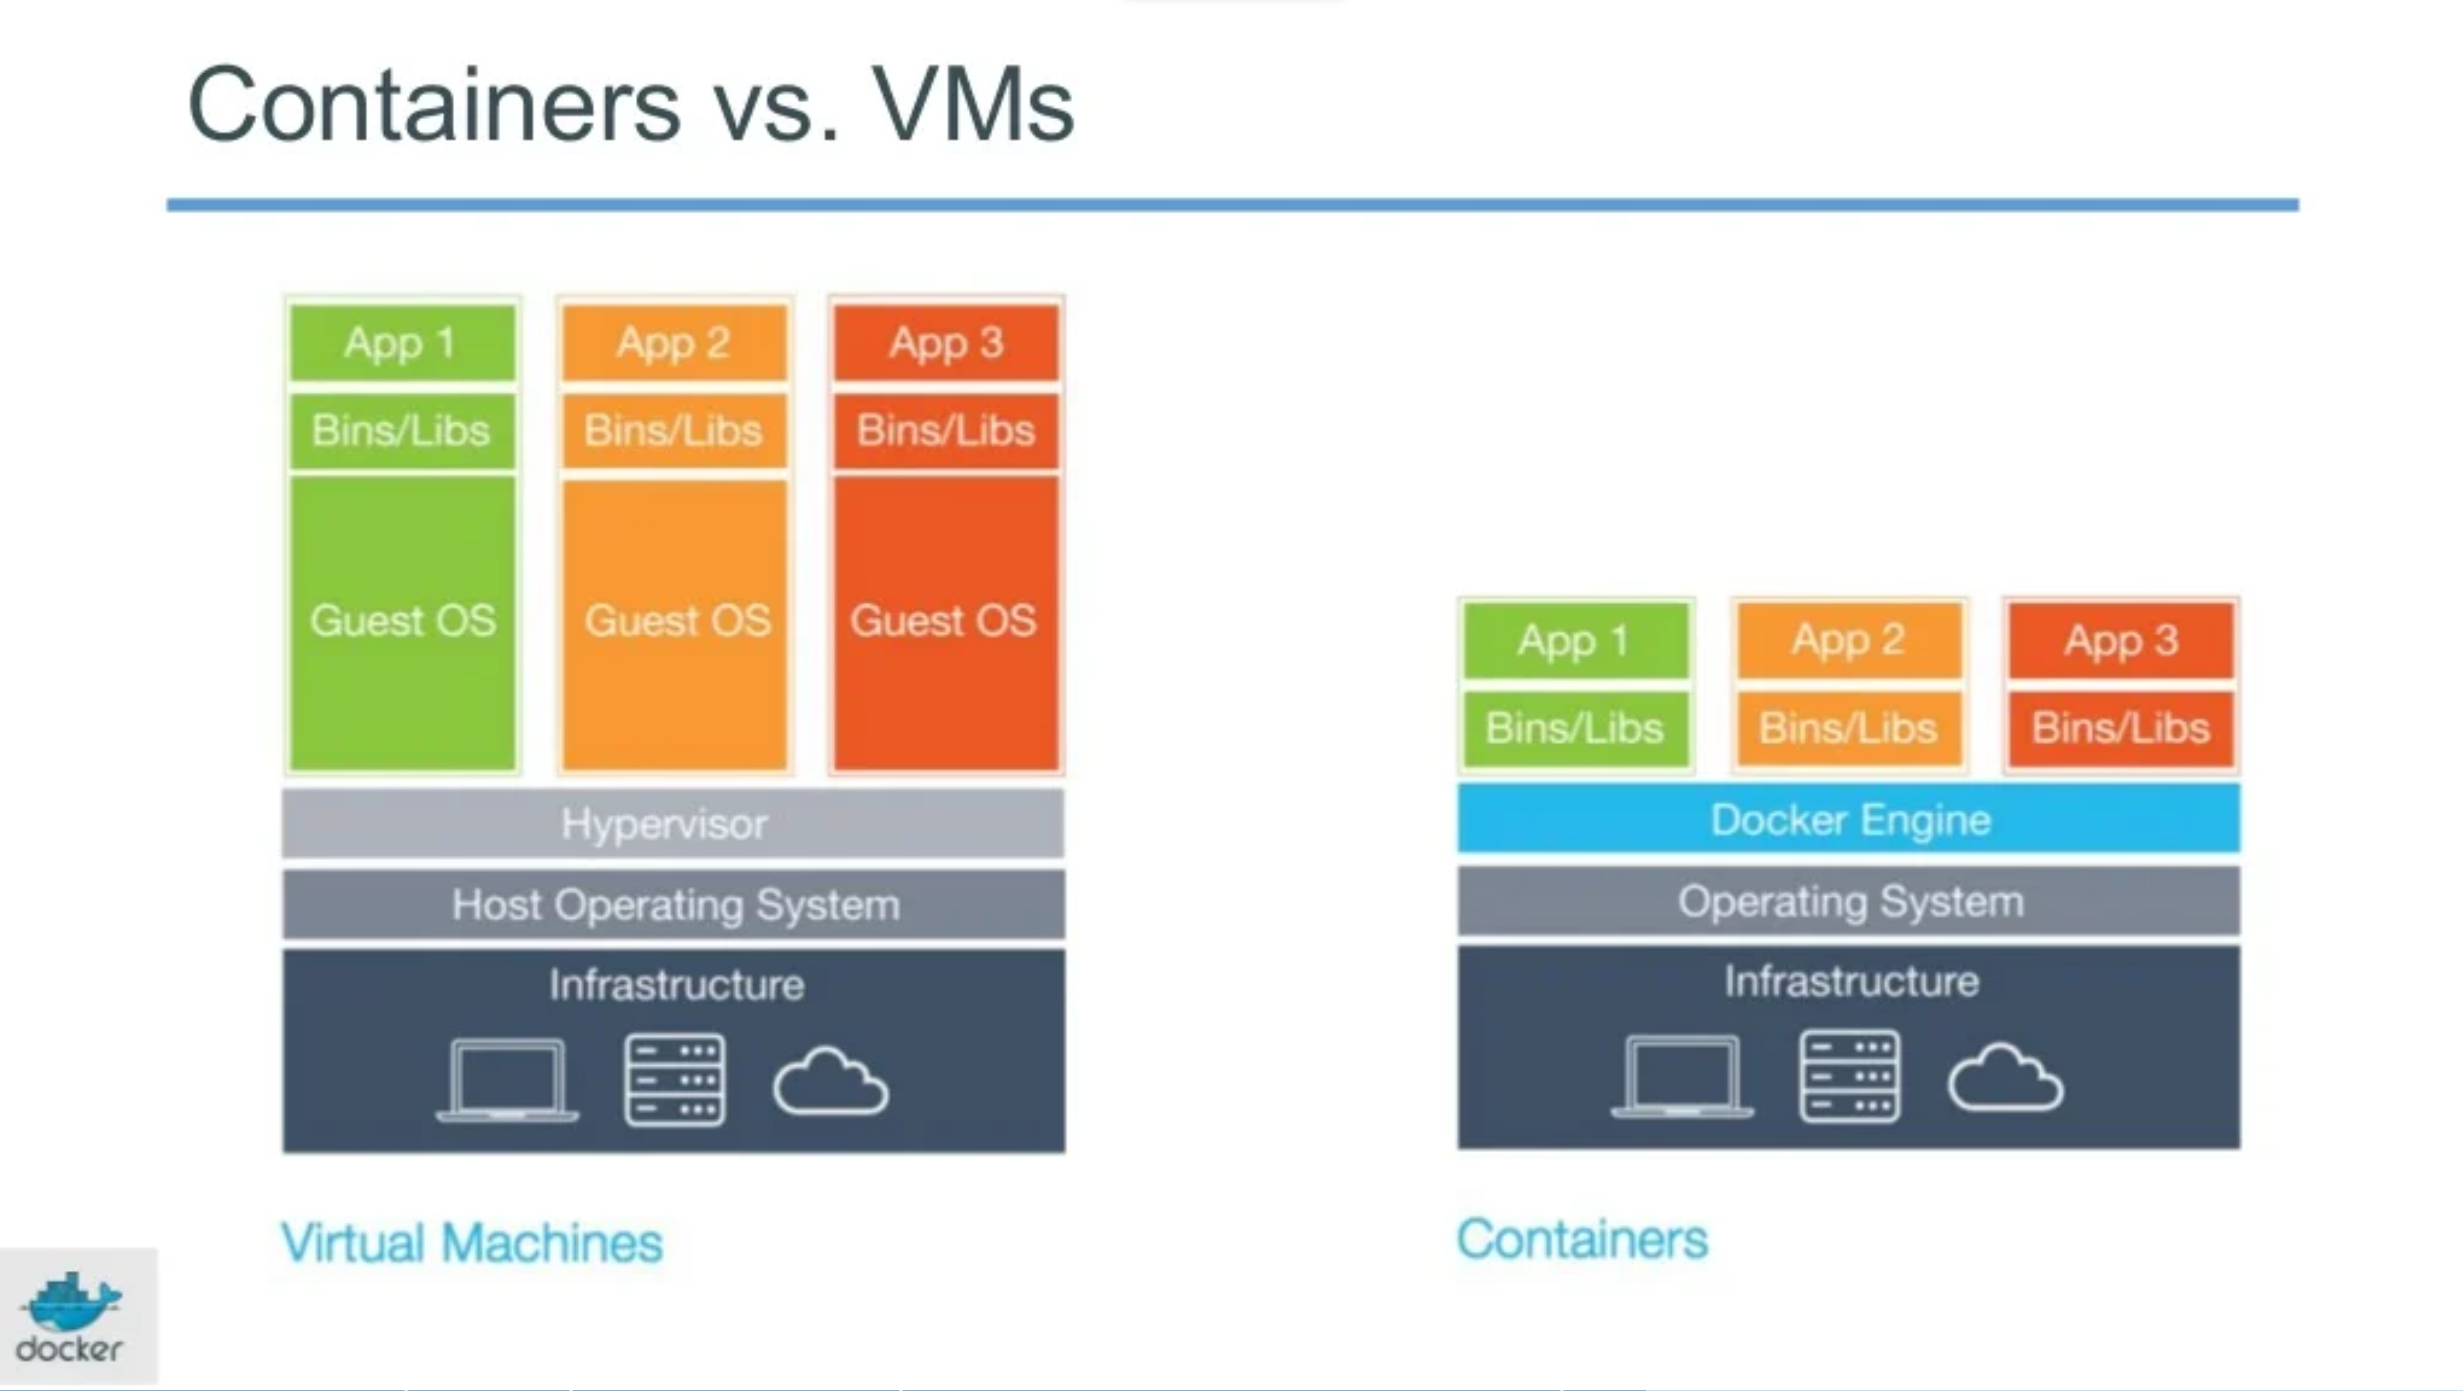
\includegraphics[width=1\textwidth]{docker_vs_vm.png}
    \caption{Docker vs. virtual machines \cite{docker:vs_vm}}
    \label{fig:dockervsvm}
\end{figure}

\section{Docker Architecture (SS)}

In this section, we will be discussing the Docker architecture and its vital components that build the technology under study. The Docker architecture is based on a client-server model where the client is called Docker client and the server is called Docker Host, see Figure \ref{fig:overview} \citep{docker:overview, aquasec:docker_architecture}. The client and the host do not necessarily need to be on the same system, as the client can communicate with the host using the Docker REST API through either a UNIX socket or a network interface. Docker images are specified in a Dockerfile, which defines the steps of how to build and run the image in a container. These built images can be stored in a private or public Docker Registry.

\begin{figure}[h]
    \centering
    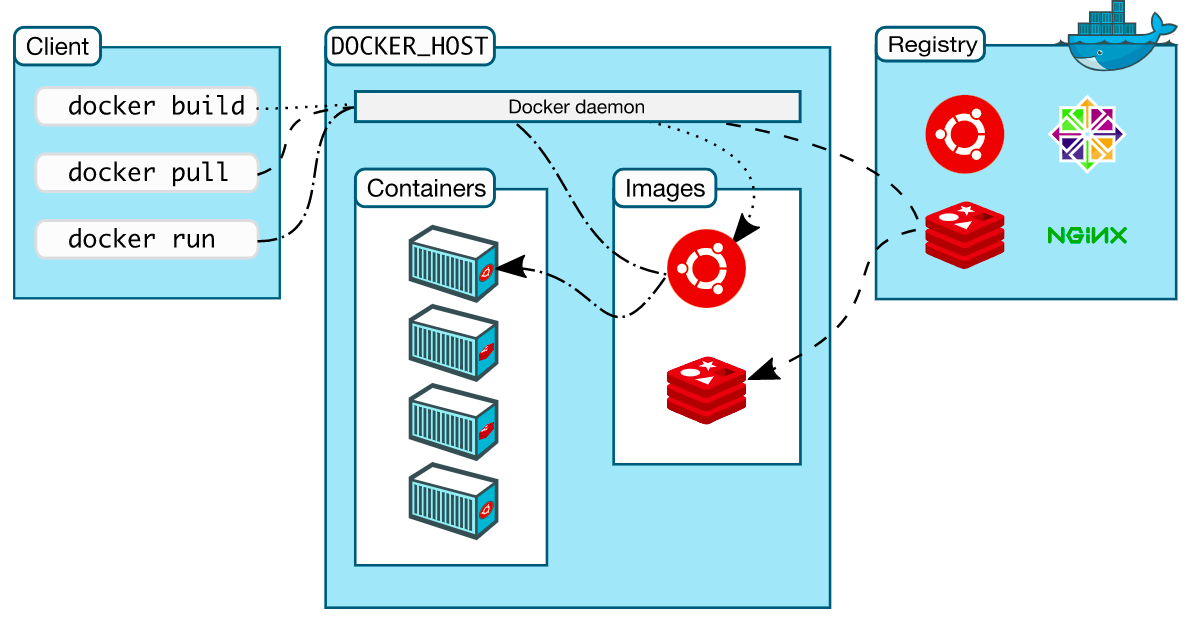
\includegraphics[width=1\textwidth]{docker-overview}
    \caption{Overview of the Docker Architecture where we can see the vital components (Client, Host, and Registry) and the sub-components they provide \citep{docker:overview}}
    \label{fig:overview}
\end{figure}

\subsection{Docker Client}

The Docker Client is the application that the user uses to interact with the Docker environment \citep{aquasec:docker_architecture}. The client provides a command-line interface (CLI) that enables the user to give commands to the Docker Hosts daemon. A client is able to communicate with many daemons.

\subsection{Docker Host}

The Docker host contains many components, such as the daemon, images, containers, networking, and storage, that provide the environment for running and executing applications \citep{aquasec:docker_architecture}. The daemon is responsible for handling container-related commands that are received from the client, such as pulling pre-built images from a registry, executing instructions defined in a Dockerfile, and building and running the containers on the server.

\subsubsection{Docker Images}

Docker Images are read-only binary files that are used to build containers \citep{docker:overview}. Images are built using a Dockerfile that defines the instructions for the daemon to execute. Each instruction creates a layer in the image built. A layer can be thought as a small image inside the larger image that is being built. If an instruction is changed in the Dockerfile the daemon will only rebuild the image on the layers affected by the change, thus speeding up the process of creating containers from slightly modified images. Once the image is built, you can run the image in a container. Each container can be saved as an image and images support versioning.

\subsubsection{Docker Containers}

Docker Containers are isolated environments that run applications \citep{aquasec:docker_architecture}. The container contains all the necessary dependencies that are required for running the application. Running containers are isolated from other containers and also have good isolation from the host machine \citep{docker:security}. Containers can be connected to networks and storage and in this way, the isolation to the host machine can be configured.

\subsubsection{Docker Networking}

Docker uses \textit{iptables} rules on Linux hosts to provide network isolation \citep{docker:iptables}. Linux iptables provide the possibility to restrict access for the Docker host, as by default, all external IPs are able to connect to a Docker host. Docker environment has several network drivers by default, such as \citep{docker:network}:

\begin{itemize}
    \item \textbf{bridge}: The default driver. Used when multiple containers on the same host need to communicate with each other.
    \item \textbf{host}: Containers use the Docker host's networking layer directly.
    \item \textbf{overlay}: Used to connect multiple Docker daemons together. Should be used if two containers are on different Docker hosts.
    \item \textbf{none}: Disables container networking.  
\end{itemize}

Docker also supports third-party network plugins, user-defined IP addressing, and defining a MAC address to a container, so the container can be seen as a physical host in the network \citep{docker:network}.

\subsubsection{Docker Storage}

Data stored within the container are non-persistent and the data will disappear once the container stops running \citep{aquasec:docker_architecture}. For persistent storage, Docker offer four options – Data Volumes, Data Volume Container, Directory Mounts and Storage plugins. 

Data volumes are located on the host's file system and can be shared with many containers. A data volume container is a dedicated container that hosts a volume from the host. Each container using the volume connects to the container that hosts the persistent storage. Using Directory mounting, a container can have access to any folder on the host and with storage plugins, containers can use persistent storage that is for example hosted on the cloud.

\subsection{Docker Registry}

A Docker registry is a service for storing and downloading images \citep{aquasec:docker_architecture}. A registry can be publicly or privately hosted. Some most known public registries are Docker Hub and Docker Cloud.

\section{Quality Attributes}

[The qualities (-ilities) that the TUS claims to support (what?) and justifications for the claims (how?)]
[Are we missing some important -ility?]

Based on how Docker is built, the system has some qualities hoisted in it. In this section, we will list some important qualities from the architectural and agile perspective, if you decide to use Docker in your infrastructure. 

\subsection{Portability (SS)}
One key aspect of Docker is its Portability. With software portability, we refer to the usability of the same software in different environments, such as the underlying operating system or hardware \citep{wiki:Software_portability}. Portability is achieved based on how the Docker technology is built. Each container includes all the dependencies required for the application to work and only requires an underlying operating system and infrastructure that supports the Docker Engine \citep{hy:DevOps_with_Docker}.

\subsection{Deployability (SS)}
As Docker images are versionable, this gives the possibility to easily test, roll back and deploy applications\citep{hentsu:benefits}. As Docker images are smaller than Virtual Machine images, deploying an image to production is fast and results in a short downtime when deploying to a production environment. 

\subsection{Security (DK)}
Docker promises some security advantages if configured correctly \citep{docker:security}:
\begin{itemize}
    \item  Docker namespace is isolated from other programs on the machine. It cannot access other software namespaces and other software cannot access Docker's namespaces. 
    \item Each container has its own network stack and doesn't get privileged access to other containers' sockets.
    \item Docker utilizes control groups. For security, this means that a single container cannot bring the machine down even if it tried to. (Performance wise)
    
\end{itemize}
[käsittele docker security research paper \citep{docker_security_paper}]

\subsection{Scalability (DK)}
Scalability is one of the main selling points of Docker and especially if bundled with microservice architecture the scalability is great. With Docker, you can easily deploy as many containers of your service as you need and even adjust the number of containers during runtime.

\subsection{Maintainability (DK)}
Docker separates all applications into their own virtual environments. With this, different applications don't interfere with other applications and each application can have all its dependencies easily and reliably every time without affecting other software. This allows different applications to use different versions of the same dependencies.

\section{Architectural impact (DK)}

[What aspect of application/system architecture is affected by using it and how?
Architectural impact - give an example of how the application/system architecture is affected by using it
https://devopswithdocker.com/part-1/1-getting-started
"Works on my machine", different versions for different containers, isolation?]

Docker is mainly a tool for development and deployment. The application itself doesn't necessarily know if it is run on a physical machine, a virtual machine, or in a Docker container. Therefore, Docker does not absolutely have any impact on the software architecture. However, Docker excels with running multiple containers at the same time easily and therefore is a great tool for developing and deploying software with microservices architecture. This leads to the fact
that constructing microservices software becomes much less cumbersome and more easily configurable, so Docker allows people to make microservices more easily, making it a great pattern to develop and test and thus has an indirect architectural impact.

[here for developtment]
[here for isolation]
[here for different versions of the same dependencies in different containers on the same software]

\section{Limitations (SS)}

As Docker adds a layer between the container and the host kernel it doesn't suit well if you need to get full performance from your underlying hardware, although it is still more lightweight than VMs\citep{cloudsavvy:not_to_use}. In comparison to virtual machines, containers are not able to run different operating systems that would require a different kernel than the underlying host machine. For simple monolith architectures and desktop applications with high graphical requirements, Docker containerization does not offer the possible qualities that the Docker orchestration and containerization provide.

[Perhaps something on architectural impact and/or more on the graphical part]

\section{Docker Tools (SS)}

Docker Engine is available on the common operating system, such as Windows, macOS, and Linux distributions, and on the most common processor architectures, i.e. x86\_64, amd64, arm, and aarch64 \cite{docker:install}.  On Windows and Mac, the Docker toolset that contains all the necessary components to run Docker is called Docker Desktop. Currently, for Linux, they are developing this same toolset as well. With the help of Docker tools, developers are able to run, terminate, build and manage images and containers easily without the need to install any additional programs to run an application on their local machine.

Docker Desktop for Windows uses the Windows Subsystem for Linux 2 (WSL2) or Hyper-V hypervisor and Windows Containers feature, which is available on the most recent versions of 64-bit Windows 10 and 11\cite{docker:windows}.

[Docker orchestration / Kubernetes / Docker swarm?]

\bibliography{sample}

\end{document}